\documentclass[review,3p,authoryear]{elsarticle}

\usepackage{amsmath}
\usepackage{amsfonts}
\usepackage{graphicx}
%\usepackage[small]{caption}
\usepackage[font=small,subrefformat=parens]{subcaption}
\usepackage{booktabs}
\usepackage{multirow}
\usepackage{rotating}
\usepackage{url}
\usepackage[table]{xcolor}
\usepackage{hyperref}
\usepackage{dblfloatfix}
\usepackage{adjustbox}

\journal{NeuroImage}

\bibliographystyle{elsarticle-harv}

\begin{document}

\begin{frontmatter}

\title{Identifying brain regions associated with virtual environment stimulus information}

\author[ECE,NS]{Andrew Floren}

\author[NS]{Bruce Naylor}

\author[CS]{Risto Miikkulainen}

\author[BCM]{David Ress\corref{cor}}
\ead{ress@bcm.edu}

\address[ECE]{Department of Electrical and Computer Engineering}
\address[NS]{Department of Neuroscience}
\address[CS]{Computer Science Department \\ The University of Texas at Austin, Austin, TX 78712 USA}
\address[BCM]{Department of Neuroscience \\ Baylor College of Medicine, Houston, TX 77030 USA}

\cortext[cor]{Corresponding author.}

\begin{abstract}
Virtual environments provide a framework for creating complex and dynamic stimuli in a controlled fashion while multivariate pattern analysis (MVPA) makes it possible to characterize the neural-processing substrate when the underlying processing model is unknown. 
Used together, virtual environments and MVPA allow for the creation of very powerful experimental designs. 
The benefits and potential pitfalls of these techniques are evaluated on the passive encoding of the number of human characters presented in a realistic and dynamic stimulus using functional magnetic resonance imaging (fMRI) data analyzed by MVPA. 
Classifiers were trained using a spatially distributed subset of stimulus-responsive voxels at each time point and their performance was estimated using multi-fold cross-validation.
A sensitivity analysis was used to identify small and spatially distributed subsets of voxels that were sufficient for decoding the number of human characters from the fMRI signal.
The discriminative models learned by MVPA had a prediction accuracy that was two to four times above chance for all subjects, demonstrating that the combination of virtual environments and MVPA is a powerful approach to identify neural substrates evoked by complex visual stimuli.
\end{abstract}

\begin{keyword}
fMRI \sep MVPA \sep machine learning \sep virtual environments\sep vision
\end{keyword}

\end{frontmatter}

\section{Introduction}
Much research using functional magnetic resonance imaging (fMRI) and the blood-oxygen-level dependent (BOLD) signal utilize static images to analyze how the brain responds to stimuli.
Such work usually focuses on a single variable of interest, and creates stimuli that attempt to isolate that variable.
While this approach has proven to be successful, it does not mimic the dynamically changing environment in which the primate brain has evolved.
More natural and dynamic stimuli will evoke a more complex network of brain responses.
The context in which a stimuli is presented will affect how it is processed, and such complex responses can make interpretation difficult.
Therefore, it is important to test whether currently accepted neural correlates of experience remain valid in more natural settings.

Researchers have been using dynamic stimuli in the form of virtual environments \citep{Maguire1998,Calhoun2002,King2006,Mathiak2006,Spiers2007a,Hassabis2009} and prerecorded movies \citep{Hasson2004,Chadwick2010,Nishimoto2011} for some time.
Virtual environments have two strong advantages over prerecorded movies: the stimulus designer has complete control over the stimuli and the subject can interact with the environment in real time.
Precise control of the environment allows for the interrogation of very subtle parameters as well as automatic coding of relevant scene parameters.
Many variables of interest, such as semantic labels for visible objects are explicitly specified by the virtual environment's design, avoiding the need to manually label each frame (as is usually done with movies).
Furthermore, subjects can interact with virtual environments in real time,  making it possible to examine learning mechanisms and decision making in a realistic context.
This interactivity can also be employed to intentionally engage and control cognitive function.

More complex stimuli require more complex analysis methods.
A wide variety of methods have been used to analyze dynamic stimuli; general linear models (GLM) including statistical parametric mapping (SPM), independent component analysis (ICA), and multivariate pattern analysis (MVPA) are among the most popular \citep{Spiers2007}.
These analysis methods can generally be split into stimulus-driven methods---such as SPM---that measure the statistical significance of a hypothesis, and data-driven methods---such as MVPA---that look for patterns in the fMRI signal.
Stimulus-driven analyses provide more easily interpretable results but become less tractable as the complexity of the stimulus increases.
Data-driven analyses, on the other hand, can cope with more complex stimuli but are more difficult to relate to brain physiology.
A hybrid approach is also possible: data-driven analyses can first uncover complex patterns evoked by realistic stimuli; the observed relationships can then help formulate hypotheses and design stimuli to be tested by stimulus-driven analyses. 
Moreover, it may also be possible to use these realistic stimulus-response relationships to better understand subject training and pathophysiology.

Although many dynamic stimuli experiments employ GLM methods \citep{Maguire1998,Calhoun2002,King2006,Mathiak2006,Spiers2007a}, there is a general trend in newer experiments to use MVPA \citep{Hassabis2009,Chadwick2010}. 
The application of MVPA analysis to virtual environments stimuli opens up an exciting range of experiments to examine complex brain responses in more realistic stimulus scenarios.
MVPA has been used as a blanket term for the application of any classification algorithm to fMRI data, although the support vector machine (SVM) is by far the most popular choice.
When applying MVPA, the stimulus is typically organized into multiple categories or classifications such as houses or faces, ambiguous or unambiguous sentences, or gratings of specific orientations \citep{Haxby2001,Mitchell2003,Haynes2006}.
The algorithm is then trained to classify the patterns of BOLD activations into these categories at a particular time-point using labeled examples.
The performance of the classifier is defined to be the probability that it will classify a previously unseen example successfully;
this measure of performance must be estimated using statistical methods.
MVPA can be applied to the whole brain as well as to small localized regions (e.g., using the ``searchlight'' technique; \cite{Kriegeskorte2006}), which can then be used to localize functional processing.
MVPA methods consider the pattern of activation of many voxels at a particular interval in time, in contrast to GLM, which treats each voxel independently as a time-series of responses over an extended period of time.
By considering multiple voxels simultaneously, MVPA has been used to identify effects that were previously thought to be too fine scale to resolve with fMRI \citep{Kamitani2005,Hassabis2009}.

In this paper, we test the feasibility of extracting complex information from fMRI data while subjects view natural and dynamic stimuli.
The experiments were structured to identify those parts of the brain that contain information about the number of human characters in a scene.
Unlike previous experiments that examined the neural correlates of object counting or number evaluation \citep{Dehaene1999,Rickard2000,Barth2006}, a passive-viewing paradigm was used.
The recent work of \cite{Harvey2013} is more similar in that the visual perception of number was explored while the subject's task was unrelated to counting.
However, that study employed simple high-contrast dots rather than dynamic objects in a three-dimensional environment.

In our experiments, classifiers were obtained using four machine-learning techniques to compare their relative performance. 
All classifiers were trained using a spatially distributed subset of stimulus-responsive voxels at each time point and their performance was estimated using multi-fold cross-validation. 
Classification accuracy was two to four times better than chance for all subjects and machine-learning techniques tested.
A novel sensitivity mapping technique was then used to identify voxels that are important for classification and thus likely to be involved in processing the information that the classifiers were trained to identify.
Results indicate that information regarding  the number of visible characters in a complex stimulus is largely encoded early in visual processing, utilizing both ventral and dorsal visual streams.
The results also  demonstrate that complex information can effectively be extracted from a realistic virtual environment stimulus paradigm, opening up new prospects for the use of virtual environments with MVPA in neuroscience.

\begin{figure*}
\centering
\begin{subfigure}{0.3\textwidth}
\centering
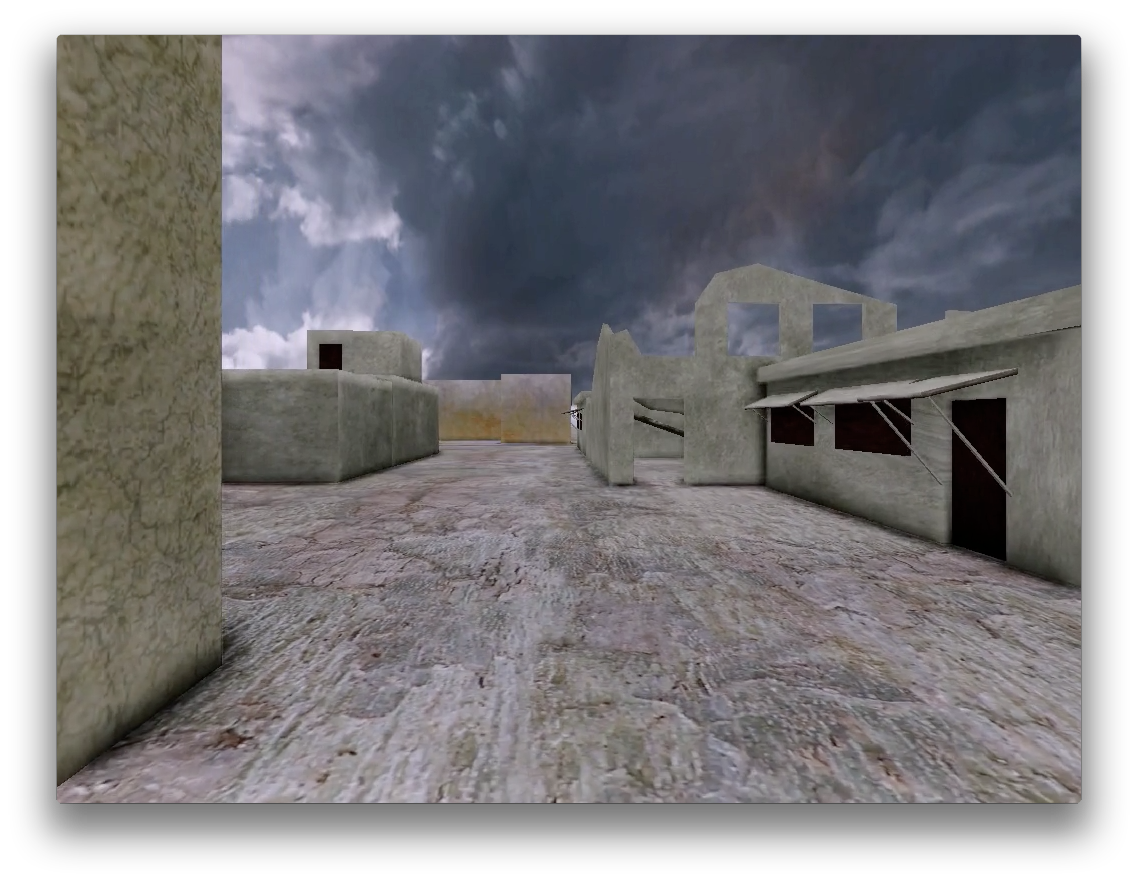
\includegraphics[width=\textwidth]{figures/stimulus-town}
\caption{}
\label{fig:stimulus-town}
\end{subfigure}
\begin{subfigure}{0.3\textwidth}
\centering
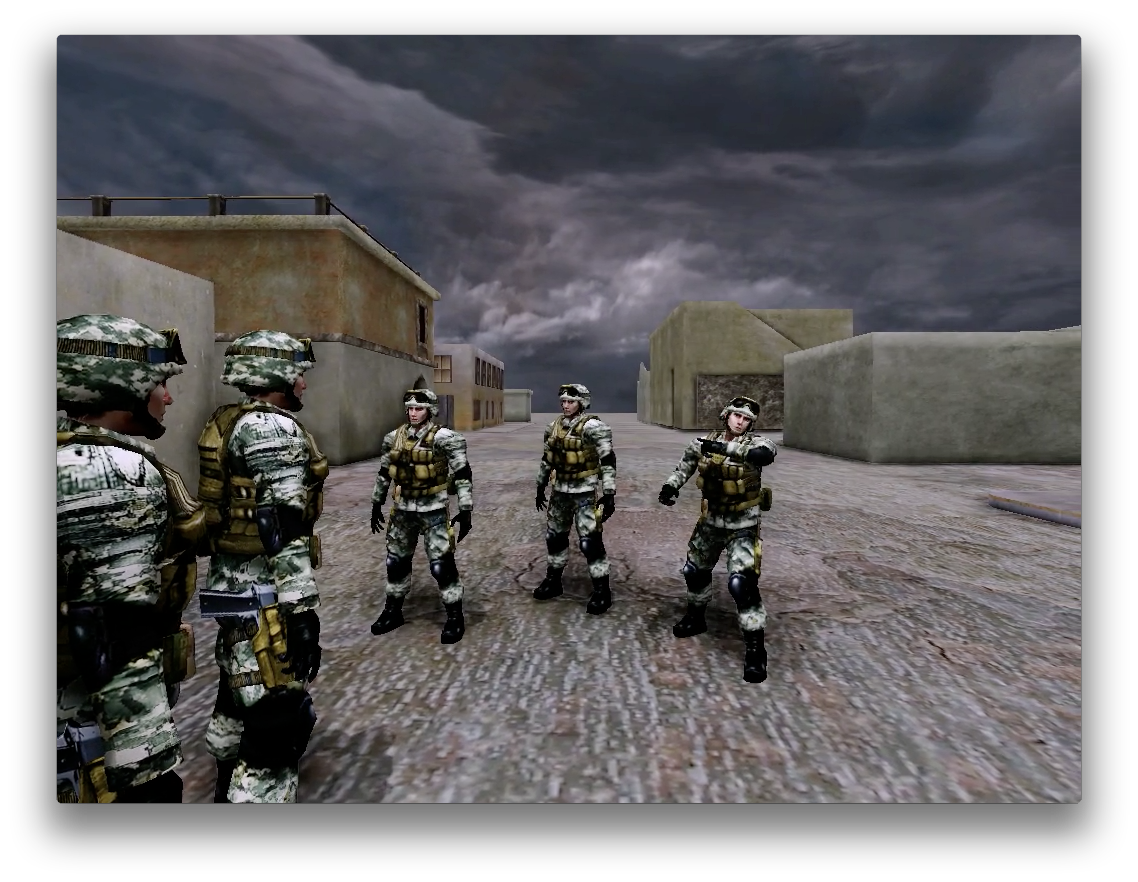
\includegraphics[width=\textwidth]{figures/stimulus-five-soldiers}
\caption{}
\label{fig:stimulus-five-soldiers}
\end{subfigure}
\begin{subfigure}{0.3\textwidth}
\centering
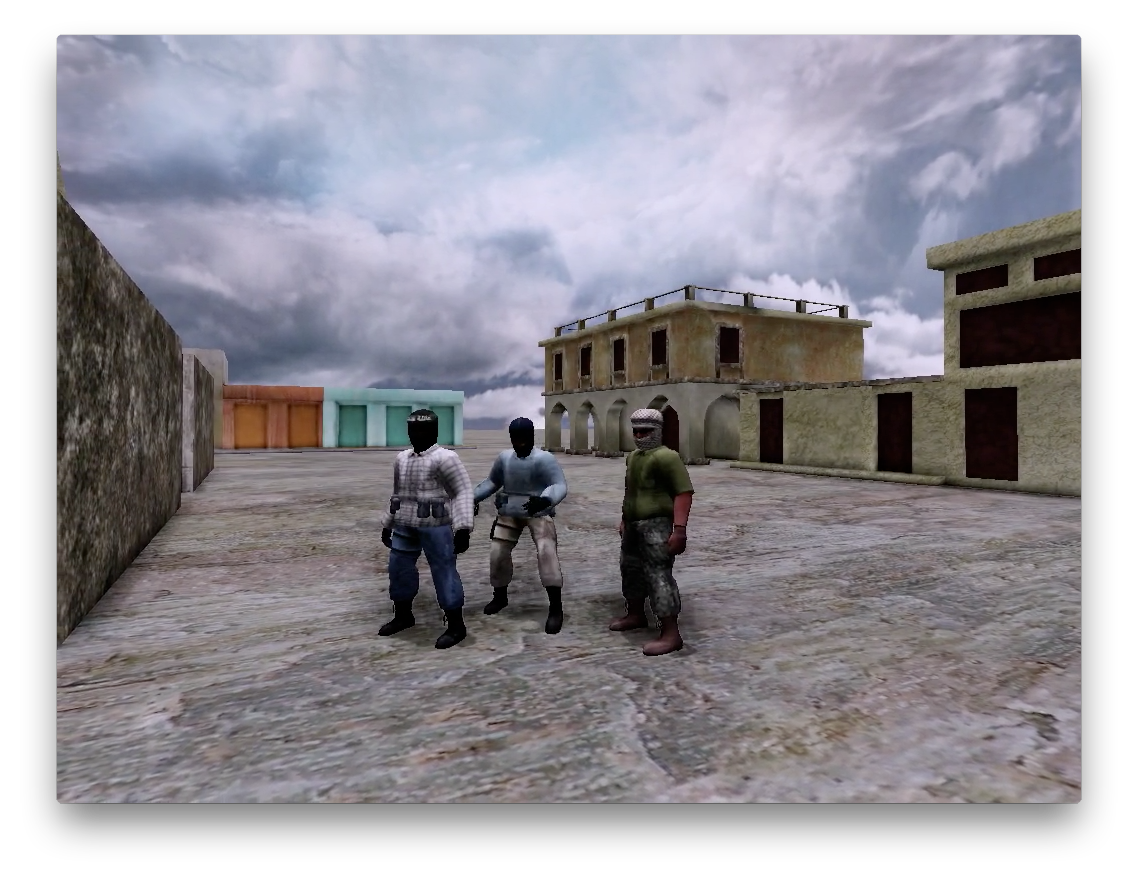
\includegraphics[width=\textwidth]{figures/stimulus-three-insurgents}
\caption{}
\label{fig:stimulus-three-insurgents}
\end{subfigure}
\caption{
The stimulus in the experiment described in this paper employs a virtual environment and a blocked design where the view alternates between moving through the environment and viewing groups of animated characters.
\subref{fig:stimulus-town} An example frame from the stimulus where the camera is traveling through the virtual environment with no characters presented.
\subref{fig:stimulus-five-soldiers} An example frame from the stimulus where five friendly characters are being presented.
\subref{fig:stimulus-three-insurgents} An example frame from the stimulus where three hostile characters are being presented.
Such stimuli allow studying how the brain respondes in a more natural and complex environment.
}
\label{fig:stimulus}
\end{figure*}

\section{Methods}

\subsection{Subjects}
Five adult males, ages 24--57, with normal or corrected-to-normal vision, participated in the experiments. 
All subjects participated in two fMRI sessions and a third session to acquire a high-resolution structural anatomy. 
Informed consent was obtained from all subjects.

\subsection{Stimulus}
To facilitate designing our virtual environment, the Unreal Developer's Kit developed by Epic Games, Inc. was used (available at \url{http://www.unrealengine.com/udk}).
This development kit is available free of charge for non-commercial applications and uses the same rendering and game engine found in many current and popular video games.

One of the long-term goals of this research is to understand post-traumatic stress disorder.
Therefore, we created a virtual town intended to mirror the kinds of real-world settings encountered by many currently deployed military forces (Fig. \ref{fig:stimulus}).
Virtual characters representing friendly forces and hostile combatants were situated at a variety of locations throughout the virtual town.
The stimulus was rendered in real-time from the point of view of a camera moving at eye level through the town. 

During the stimulus presentation, the camera followed a preset path through the town.
The stimulus employed a blocked approach. The camera would be steadily moving for 15 seconds, followed by 15 seconds in which it stopped to view virtual characters at predefined locations.
There were four different predefined character-viewing locations, and the number of characters present at each of these locations varied from one to six (Figs. \ref{fig:stimulus-five-soldiers} and \ref{fig:stimulus-three-insurgents}).
While the camera was stopped to view the characters, the view slowly panned and rotated and the characters engaged in animated movement sequences, so that the scene was never static.
A passive viewing paradigm was employed for this stimulus: there was no fixation dot and no task during the presentation.

Scanning sessions included five to six runs that were six minutes in duration.
Each run contained 12 alternations between moving through the virtual environment and character presentations. 
Since there were four predefined character viewing locations, the camera made three laps around the town during a single run.
While the number of characters presented in each block varied from one to six, the stimulus was controlled such that a presentation with a particular number of characters appeared twice in each run.
The ordering of the presentations was also controlled such that presentations with the same number of characters were located at different viewing points.
The order of the presentations was generated randomly given the previous constraints, but the same ordering was used for each subject.
A single type of character (friend or foe) was presented in each run, and character type was alternated from run to run.

\subsection{MRI protocols}
Imaging was performed on a GE Signa Excite HD scanner using the product eight-channel head coil.
Whole-brain image volumes were collected using a custom GRAPPA EPI sequence \citep{Griswold2002}. 
Sequence parameters were g-factor = 2,  TE = 25 ms, TR = 2.5 s, and  2.5-mm cubic voxels across a 200 mm field-of-view. 
The slice prescription included 40 slices oriented along the AC-PC axis. 
A high-order shim was  performed to improve field homogeneity.

A set of T1-weighted structural images was obtained on the same prescription before the functional acquisition runs using a three-dimensional (3D) fast RF-spoiled GRASS (fSPGR) sequence. 
These anatomical images were then used to align the functional data to a structural 3D reference volume, which was acquired for each subject in a separate session. 
The structural reference volume was T1-weighted with good gray-white contrast and was acquired using a 3D inversion-prepared fSPGR sequence (minimum TE and TR, TI = 450 ms, 15$^\circ$ flip angle, isometric voxel size of 0.7 mm, 2 excitations, $\sim$28-minute duration).

\subsection{Preprocessing}
Preprocessing of the fMRI data was performed using the mrVista software package (available at \url{http://vistalab.stanford.edu/}). 
The first 15 seconds of data  were discarded to reduce transient effects.
Within-scan motion was then estimated using a robust intensity-based scheme \citep{Nestares2000}. 
Between-run motion was corrected using the same scheme, this time applied to the temporal average intensity of the entire scan. 
The first run of the session was used as the reference. 
Because the goal is to learn associations between patterns of activation in the brain and stimulus presentation, it is important that the activation is temporally aligned with the stimulus.
Therefore, a Wiener filter deconvolution \citep{Poor1980} was applied using a generic difference-of-gamma hemodynamic response function (HRF; \cite{Glover1999}) as the kernel to the recorded BOLD signal.
Mostly, the deconvolution served to shift the peak response in time so that it was aligned with its associated stimulus, but it also provided some amount of noise reduction.

In Wiener filter deconvolution, the deconvolution kernel $g(t)$ is most easily expressed in the Fourier domain as
\begin{equation}
g(t) \xrightarrow{\mathcal{F}} \frac{H^{*}(f)}{\left|H(f)^{2}\right| + \frac{\left| N(f) \right|}{\left| X(f) \right|}},
\end{equation}
where $h(t)$ is the blurring kernel, $x(t)$ is the signal of interest, and $n(t)$ is additive noise; capital letters denote the Fourier transform of each quantity, e.g., $h(t) \xrightarrow{\mathcal{F}} H(f)$.

In fMRI, $h(t)$ is the hemodynamic response function and $x(t)$ is the neural response.
Calculating $g(t)$ requires estimates of the power spectral density of the signal of interest as well as the noise.
However, the noise $n(t)$ corresponds not only to scanner noise but other nuisance factors such as pulse and respiration.
These factors make modeling the noise, and its power spectral density, very difficult.
Therefore, $\frac{\left| N(f) \right|}{\left| X(f) \right|}$ was set to $1.0$, a compromise value that provided a satisfactory combination of temporal alignment and noise reduction for all subjects.

The high-resolution reference anatomies were segmented using the Freesurfer image analysis suite (\url{http://surfer.nmr.mgh.harvard.edu/}) to create approximate parcellations of the gray matter in each subject, as well as a surface model useful for visualization of the results.

\subsection{Dimensionality reduction}
When performing MVPA, each voxel can be thought of as corresponding to a separate dimension of a very high-dimensional space.
For this experiment's acquisition parameters, the number of voxels/dimensions was $80 \times 80 \times 40 = 256,000$.
Because the number of examples necessary to train a classifier increases rapidly with the number of dimensions, it was useful to reduce this dimensionality.
This reduction not only speeded up both training and classification but also improved the performance of the resulting classifiers.

Principal component analysis (PCA; \cite{Hotelling1933}) is a common tool for dimensionality reduction.
However, PCA only selects the orthogonal dimensions with the highest variance, which are likely to include physiological nuisance and such approaches are therefore not well suited for fMRI analysis.
Univariate statistical methods, as typically used in  fMRI analysis, can also be good candidates for selecting voxels \citep{Norman2006,Pereira2009}.
While effective, these methods were not designed for feature selection and many of them make a number of assumptions about the data such as a Gaussian statistical distribution.

A novel method of dimensionality reduction was developed in this research.
This method, called harmonic analysis, selects voxels that are driven most strongly by the 30-second duty cycle of the block design.
This method is similar to other univariate statistics, but the only assumption is that the BOLD response is linear with respect to the stimulus.
The primary advantage is that it can detect voxels that covary with the stimulus regardless of their detailed temporal relationship. 
Thus, it includes voxels that respond positively to either the character presentation or motional phases of the stimulus alternation, or to more complex patterns such as a brief strong response to both phases. 
All repetitive responses that follow the period of the stimulus alternation are included by this method, minimizing any bias in the dimension reduction.

Harmonic analysis takes advantage of the fact that the response of any linear system to a blocked alternation at frequency $f$ will contain power only at $f$ and its harmonics. 
Under a linear response assumption, we can therefore form an unbiased estimate of the response power by summing the power at these frequencies. 
Let $y(t)$ be the recorded discrete time series at some voxel.
Then let $Y(f)$ be the discrete Fourier transform of $y(t)$.
The fractional harmonic power of that time series is defined as
\begin{equation}
P_h = \frac{\sum_{i = 1}^{M}{\left|Y(i \cdot N)\right|^{2}}}{\sum_{f}{\left|Y(f)\right|^{2}}},
\end{equation}
where $P_h$ is the fractional harmonic power, $M$ is the number of harmonics, and $N$ is the frequency of interest, in our case the period of the block alternations. 
Because the BOLD response has a predominantly low-pass temporal frequency response, we chose $M = 4$ as sufficient. 
Using $P_h$, a particular number, $N = 2000$, voxels with the greatest power are selected. 

This harmonic-power selection was based on the alternation between characters present and characters absent, without regard to the number of characters presented. 
Therefore, classifier accuracy estimates will only be presented for character count, and not for the presence or absence of characters, in order to avoid overlap between dimension-reduction and  classification criteria that would result in inflated classifier performance estimates \citep{Pereira2009}.
However, the classifiers were also trained to distinguish between time points with and without characters as a check, and their performance was consistently above 95\%, confirming that the machine-learning algorithms were working correctly.

\subsection{Classification}
Using the time series from the voxels selected by the harmonic analysis, a one-versus-one multi-class linear support vector machine (SVM) \citep{Cortes1995,Weston1999}, a feedforward neural network (NN) \citep{Hornik1989,Hagan1994}, a Gaussian naive Bayes classifier (GNB) \citep{Duda1973}, and a k-nearest neighbor classifier (KNN) \citep{Cover1967} were trained to identify the number of characters presented in each scene, regardless of character type (friend or foe).
To maximize temporal resolution, each 2.5-second frame (time point) was treated as a separate example, rather than averaging across the 15-second blocks.
Similar methods were also used to classify scenes as friends or foes, but these classifiers did not perform significantly above chance and will not be mentioned further.

The performance of machine learning algorithms is generally defined to be the expected accuracy of the classifier on previously unseen examples \citep{Bishop2006}.
In practice, this measure can only be estimated.
A typical approach is to split the available examples into training and test sets.
The classifier is first trained on the training set, and its performance on the test set is then taken as the estimate.
The process of splitting all of the available examples into training and test sets is performed multiple ($n$; typically 10) times to reduce the variance of the performance estimate.
This procedure is known as $n$-fold cross-validation \citep{Kohavi1995}.
Previous studies have discussed issues with optimistically biased performance estimates due to temporal correlations that violate independence assumptions between training and test set samples \citep{Pereira2009}. 
The slow speed of the fMRI hemodynamic response clearly introduces temporal correlations on time scales less than 10 seconds.
Therefore, training and test sets were constructed by randomly drawing 15 second blocks rather than individual frames after which 10-fold cross-validation was performed.

Furthermore, the null distribution for the cross-validated performance estimates was generated by randomly permuting the labels on the examples 2000 times and repeating the training and cross-validation procedure.
That is, the distribution of performance estimates was generated under the assumption that the labels and data were independent.
Using this distribution, $p$ values were calculated for the performance estimates.
The high-performance computing resources of the Texas Advanced Computing Center (TACC) at The University of Texas at Austin were utilized to perform this computation.

\subsection{Sensitivity Analysis}
MVPA can tell us whether the time-series data from a subset of human brain voxels can be used to discriminate character number from the stimuli. 
However, these results do not show which voxels in the large group were actually important for that discrimination.
This information is important for localizing functions in the brain.
One existing technique is to train machine learning classifiers on small localized areas in the brain and use their performance as a measure of the strength of the function in question in that area; this is known as the ``searchlight'' technique \citep{Kriegeskorte2006}.
While this technique is effective for brain functions already known to be highly localized, the results are less clear when the function is sparsely distributed over the brain.
A single region may not contain enough information for accurate classification or a region may only contain relavant information only when considered in conjunction with a spatially disparate region.

To overcome this limitation, a sensitivity analysis technique originally used to minimize the input data dimension of feedforward neural networks \citep{Zurada1994} was adapted to display the spatially distributed set of voxels that are most important for identifying the classes.
Specifically, the sensitivity, or magnitude of change, of the neural network output was calculated with respect to a change in each voxel.
Let $\mathbf{o}$ be the vector of outputs and $\mathbf{x}$ be the vector of inputs.
Then the sensitivity of output $k$ to input $i$ is defined by
\begin{equation}
S_{ki} = \frac{\delta o_{k}}{\delta x_{i}},
\end{equation}
which is the partial derivative of the output with respect to the input.
Let $\mathbf{w}$ be the weight matrix from the hidden layer to the output layer and $\mathbf{v}$ be the weight matrix from the input layer to the hidden layer.
Then the partial derivative can be expressed as
\begin{equation}
\frac{\delta o_{k}}{\delta x_{i}} = o'_{k} \sum^{J}_{j=1}{w_{kj}y'_{j}v_{ji}},
\end{equation}
where $J$ is the total number of hidden units in that layer of the neural network,  $o'_{k}$ is the value of the derivative of the activation function at output $k$, and $y'_{j}$ is the value of the derivative of the activation function at hidden neuron $j$.
Finally, the entire sensitivity matrix can be expressed in matrix notation as,
\begin{equation}
\mathbf{S} = \mathbf{O}' \times \mathbf{W} \times \mathbf{Y}' \times \mathbf{V}
\end{equation}
where
\begin{equation}
\mathbf{O}' = diag(o'_{1},~o'_{2},~\cdots,~o'_{K})
\end{equation}
\begin{equation}
\mathbf{Y}' = diag(y'_{1},~y'_{2},~\cdots,~y'_{K}).
\end{equation}
However, because the transfer functions are nonlinear they can only be evaluated for specific input values.
Therefore, we calculated the average sensitivity matrix across all input vectors,
\begin{equation}
\mathbf{S}_{avg} = \sqrt{ \frac{ \sum_{n = 1}^{N}{ \left( \mathbf{S}_{n}\right)^{2} } }{N} },
\label{eqn:sensitivity}
\end{equation}
where $N$ is the number of input vectors.
The magnitude is squared so that the effects of both positive and negative sensitivities are included in the average.
Eq. \ref{eqn:sensitivity} gives a sensitivity value for each voxel with respect to every output, whereas it is useful to have a measure of the sensitivity of a voxel with respect to any output.
Such a metric can be defined by taking the maximum sensitivity of each voxel across all outputs, i.e.
\begin{equation}
\Phi_{i} = \max_{k=1 \dots K}{S_{ki,~avg}}.
\end{equation}
This sensitivity can now be projected back into the volume anatomy space to create a  map that reflects the relative incremental importance of each voxel's response to the classification decision.
In theory, a similar technique could be introduced for any differentiable classifier such as the SVM.
However, only the sensitivity analysis applied to neural networks will be presented and discussed as it has been well studied in the existing literature \citep{Zurada1994}.

We  explored the relationship between sensitivity and classifier performance by training the classifier on only a subset of the input voxels as determined by a minimum-sensitivity threshold.
The threshold was gradually increased until classifier performance was significantly degraded.

The Freesurfer image analysis suite was employed to construct cortical surfaces for each of the subjects using high-resolution anatomy volumes.
Ten anatomical labels were constructed on each surface based on FreeSurfer's automatically generated labels.
Each subject's volume sensitivity map was then projected onto their cortical surface and blurred along the surface using a 5 mm full-width half-maximum (FWHM) Gaussian kernel.
Group averaged sensitivity maps were also formed using both affine and non-linear registration algorithms.
However, the quality of the registration between our subject brains was not satisfactory.
In particular, group-average maps tended to mislocalize temporal-lobe activity onto the parietal lobe.
Therefore, sensitivity maps will be only presented on individual subject brain surfaces.
However, the total sensitivity in each anatomical label was averaged across subjects in order to examine group-average sensitivity without requiring registration.

\subsection{GLM}
GLM analysis was also performed on the data to compare classification performance and the spatial distribution of significant voxels with the MVPA sensitivity analysis maps. 
A linear activation model was constructed using an explanatory variable for each character count.
Processing of fMRI data was carried out using FEAT (FMRI Expert Analysis Tool) Version 5.98, part of FSL (FMRIB's Software Library, \url{www.fmrib.ox.ac.uk/fsl}). 
Z (Gaussianized T/F) statistic images were thresholded using clusters determined by $Z > 2.3$ and a (corrected) cluster significant threshold of $P = 0.05$ \citep{Worsley2001}.
Clusters in these images indicate regions where the magnitude of activation is linearly correlated with the number of characters presented.
The thresholded Z statistic images were projected onto the same Freesurfer generated surfaces as the sensitivity analysis.

For each voxel above the significance threshold, this model was used to construct a simple linear estimator for the number of characters presented by fitting a line to the parameter estimates of each explanatory variable versus their corresponding character counts.
A continuous estimate of character count was obtained for each frame using the linear fit and the current parameter value.
This character count estimate was clipped between one and six, averaged across significant voxels, and then rounded to the nearest whole number.
The accuracy of this model was calculated for comparison with the machine-learning techniques.

\section{Results}
The cross-validated performance estimates for nearly every session from all five subjects and all four classifiers are above chance at 16.7\% (Figure \ref{fig:performance}).
However, the cross-validated performance estimates produced by the neural network for two sessions fell to chance.
There is variation in performance between sessions for the same subject, as well as variation in average performance between subjects.
Averaged across all 10 sessions (five subjects with two sessions each), the cross-validated performance estimates of all four classifiers are significantly above chance.
The 68\% confidence intervals used for determining significance were obtained by bootstrapping across all sessions.
The SVM had the best performance overall, followed by the feedforward neural network.
The performance of all four independent classifiers being above chance increases confidence in the results, however the GNB and KNN classifiers will not be discussed further as their performance was significantly below the SVM and NN.
The average performance of the linear estimator for each session after thresholding was 29\%, roughly similar to the performance of the KNN classifier.

\begin{figure}
\centering
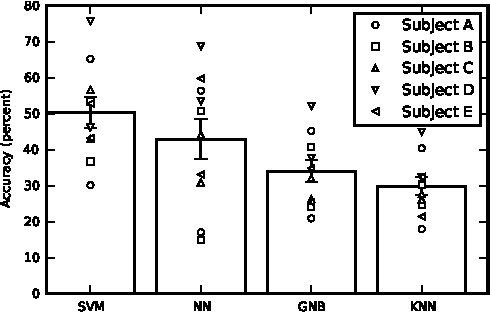
\includegraphics{figures/performance}
\caption{The estimated performace of all four classifiers averaged across all sessions.
The performances estimates were bootstrapped across sessions in order to obtain 68\% confidence intervals.
While the SVM had the best average performance, all four classifiers performed well above a chance performance of 16.7\%.}
\label{fig:performance}
\end{figure}

The average confusion matrix gives an intuitive look at the performance of the classifiers (Figure \ref{fig:average-confusion}).
The classifiers are much better at detecting the presence of a single character than any other count.
In fact, there are almost no cases of confusion between one and two characters.
Apparently, these two situations evoke very different responses in the brain.
The rest of the character counts are distinguished with relatively equal accuracy,
except for a slightly larger tendency to mis-classify the six character presentation.
Note that the majority of the incorrect responses lay just off the main diagonal.
These responses correspond to the classifier being wrong by a single character in its classification.
For example, in 21\% of the test examples, both the SVM and NN algorithms classified a frame as containing four characters when it only contained three characters.

\begin{figure}
\centering
\begin{subfigure}{0.3\textwidth}
\centering
\begin{adjustbox}{center}

\begin{tabular}{*{9}{c}}
& & \multicolumn{6}{c}{predicted count} & \\
& & 1 & 2 & 3 & 4 & 5 & 6 & \\
\multirow{6}{*}{\begin{sideways}actual count\end{sideways}}
& 1 & \cellcolor[rgb]{0.000000,1.000000,0.000000}75\% & \cellcolor[rgb]{0.987315,0.012685,0.000000}6\% & \cellcolor[rgb]{0.967214,0.032786,0.000000}8\% & \cellcolor[rgb]{0.995154,0.004846,0.000000}3\% & \cellcolor[rgb]{0.996400,0.003600,0.000000}3\% & \cellcolor[rgb]{0.991856,0.008144,0.000000}5\% & \cellcolor[rgb]{0.000000,1.000000,0.000000}71\%\\
& 2 & \cellcolor[rgb]{0.984543,0.015457,0.000000}6\% & \cellcolor[rgb]{0.000001,0.999999,0.000000}52\% & \cellcolor[rgb]{0.960568,0.039432,0.000000}9\% & \cellcolor[rgb]{0.793233,0.206767,0.000000}13\% & \cellcolor[rgb]{0.989269,0.010731,0.000000}5\% & \cellcolor[rgb]{0.754492,0.245508,0.000000}14\% & \cellcolor[rgb]{0.000002,0.999998,0.000000}50\%\\
& 3 & \cellcolor[rgb]{0.976984,0.023016,0.000000}7\% & \cellcolor[rgb]{0.946464,0.053536,0.000000}9\% & \cellcolor[rgb]{0.000000,1.000000,0.000000}53\% & \cellcolor[rgb]{0.228780,0.771220,0.000000}20\% & \cellcolor[rgb]{0.980048,0.019952,0.000000}7\% & \cellcolor[rgb]{0.995294,0.004706,0.000000}3\% & \cellcolor[rgb]{0.000001,0.999999,0.000000}51\%\\
& 4 & \cellcolor[rgb]{0.992536,0.007464,0.000000}4\% & \cellcolor[rgb]{0.888490,0.111510,0.000000}11\% & \cellcolor[rgb]{0.154156,0.845844,0.000000}21\% & \cellcolor[rgb]{0.000336,0.999664,0.000000}37\% & \cellcolor[rgb]{0.500333,0.499667,0.000000}17\% & \cellcolor[rgb]{0.939464,0.060536,0.000000}10\% & \cellcolor[rgb]{0.000499,0.999501,0.000000}36\%\\
& 5 & \cellcolor[rgb]{0.995930,0.004070,0.000000}3\% & \cellcolor[rgb]{0.976984,0.023016,0.000000}7\% & \cellcolor[rgb]{0.934220,0.065780,0.000000}10\% & \cellcolor[rgb]{0.299381,0.700619,0.000000}19\% & \cellcolor[rgb]{0.000001,0.999999,0.000000}50\% & \cellcolor[rgb]{0.919415,0.080585,0.000000}11\% & \cellcolor[rgb]{0.000000,1.000000,0.000000}55\%\\
& 6 & \cellcolor[rgb]{0.917261,0.082739,0.000000}11\% & \cellcolor[rgb]{0.217071,0.782929,0.000000}20\% & \cellcolor[rgb]{0.994473,0.005527,0.000000}4\% & \cellcolor[rgb]{0.888730,0.111270,0.000000}11\% & \cellcolor[rgb]{0.880363,0.119637,0.000000}12\% & \cellcolor[rgb]{0.000031,0.999969,0.000000}43\% & \cellcolor[rgb]{0.000004,0.999996,0.000000}48\%\\
&   & \cellcolor[rgb]{0.000000,1.000000,0.000000}75\% & \cellcolor[rgb]{0.000001,0.999999,0.000000}52\% & \cellcolor[rgb]{0.000000,1.000000,0.000000}53\% & \cellcolor[rgb]{0.000336,0.999664,0.000000}37\% & \cellcolor[rgb]{0.000001,0.999999,0.000000}50\% & \cellcolor[rgb]{0.000031,0.999969,0.000000}43\% & \cellcolor[rgb]{0.000001,0.999999,0.000000}52\%\\
\end{tabular}

\end{adjustbox}
\caption{}
\label{fig:average-confusion-svm}
\end{subfigure}
\\
\begin{subfigure}{0.3\textwidth}
\centering
\begin{adjustbox}{center}

\begin{tabular}{*{8}{c}}
& & \multicolumn{6}{c}{predicted count} \\
& & 1 & 2 & 3 & 4 & 5 & 6 \\
\multirow{6}{*}{\begin{sideways}actual count\end{sideways}}
& 1 & \cellcolor[rgb]{0.000000,1.000000,0.000000}62\% & \cellcolor[rgb]{0.975443,0.024557,0.000000}7\% & \cellcolor[rgb]{0.841309,0.158691,0.000000}12\% & \cellcolor[rgb]{0.971887,0.028113,0.000000}8\% & \cellcolor[rgb]{0.997938,0.002062,0.000000}1\% & \cellcolor[rgb]{0.960675,0.039325,0.000000}9\%\\
& 2 & \cellcolor[rgb]{0.933406,0.066594,0.000000}10\% & \cellcolor[rgb]{0.000009,0.999991,0.000000}46\% & \cellcolor[rgb]{0.933406,0.066594,0.000000}10\% & \cellcolor[rgb]{0.831816,0.168184,0.000000}13\% & \cellcolor[rgb]{0.989177,0.010823,0.000000}5\% & \cellcolor[rgb]{0.569328,0.430672,0.000000}16\%\\
& 3 & \cellcolor[rgb]{0.979969,0.020031,0.000000}7\% & \cellcolor[rgb]{0.960675,0.039325,0.000000}9\% & \cellcolor[rgb]{0.000018,0.999982,0.000000}44\% & \cellcolor[rgb]{0.071219,0.928781,0.000000}23\% & \cellcolor[rgb]{0.984753,0.015247,0.000000}6\% & \cellcolor[rgb]{0.902345,0.097655,0.000000}11\%\\
& 4 & \cellcolor[rgb]{0.989896,0.010104,0.000000}5\% & \cellcolor[rgb]{0.919227,0.080773,0.000000}11\% & \cellcolor[rgb]{0.159047,0.840953,0.000000}21\% & \cellcolor[rgb]{0.001187,0.998813,0.000000}34\% & \cellcolor[rgb]{0.739428,0.260572,0.000000}14\% & \cellcolor[rgb]{0.586267,0.413733,0.000000}16\%\\
& 5 & \cellcolor[rgb]{0.990567,0.009433,0.000000}5\% & \cellcolor[rgb]{0.971887,0.028113,0.000000}8\% & \cellcolor[rgb]{0.933406,0.066594,0.000000}10\% & \cellcolor[rgb]{0.333341,0.666659,0.000000}18\% & \cellcolor[rgb]{0.000017,0.999983,0.000000}44\% & \cellcolor[rgb]{0.697341,0.302659,0.000000}15\%\\
& 6 & \cellcolor[rgb]{0.945244,0.054756,0.000000}10\% & \cellcolor[rgb]{0.811482,0.188518,0.000000}13\% & \cellcolor[rgb]{0.937595,0.062405,0.000000}10\% & \cellcolor[rgb]{0.667251,0.332749,0.000000}15\% & \cellcolor[rgb]{0.902345,0.097655,0.000000}11\% & \cellcolor[rgb]{0.000049,0.999951,0.000000}41\%\\
\end{tabular}

\end{adjustbox}
\caption{}
\label{fig:average-confusion-nn}
\end{subfigure}
\caption{The average confusion matrices for the \subref{fig:average-confusion-svm} SVM and \subref{fig:average-confusion-nn} neural network classifiers across all subjects.
The value in cell $(i,j)$ of the matrix is the percent of examples from class $i$ that were labeled as class $j$; values along the diagonal indicate correctly classified examples while the rest indicate incorrectly classified examples.
The color of the cell indicates deviation from chance probability (16.7\%);
greener cells indicating values above chance, and redder cells indicating values below chance.
These confusion matrices show that the SVM and NN were able to distinguish all six possible character counts, but as the number of characters rose the performance tended to decrease.}
\label{fig:average-confusion}
\end{figure}

The effects of using the sensitivity analysis to further reduce voxel number was studied using the iterative retraining approach (see Methods).
As voxels are removed, performance first shows a non-significant increase to a peak when $\sim$35\% of the voxels are removed.
Performance then gradually decreases (Figure \ref{fig:sensitivity-cutoff}), but the estimated performance of the classifier was not significantly affected until over 90\% of the voxels were removed.

\begin{figure}
\centering
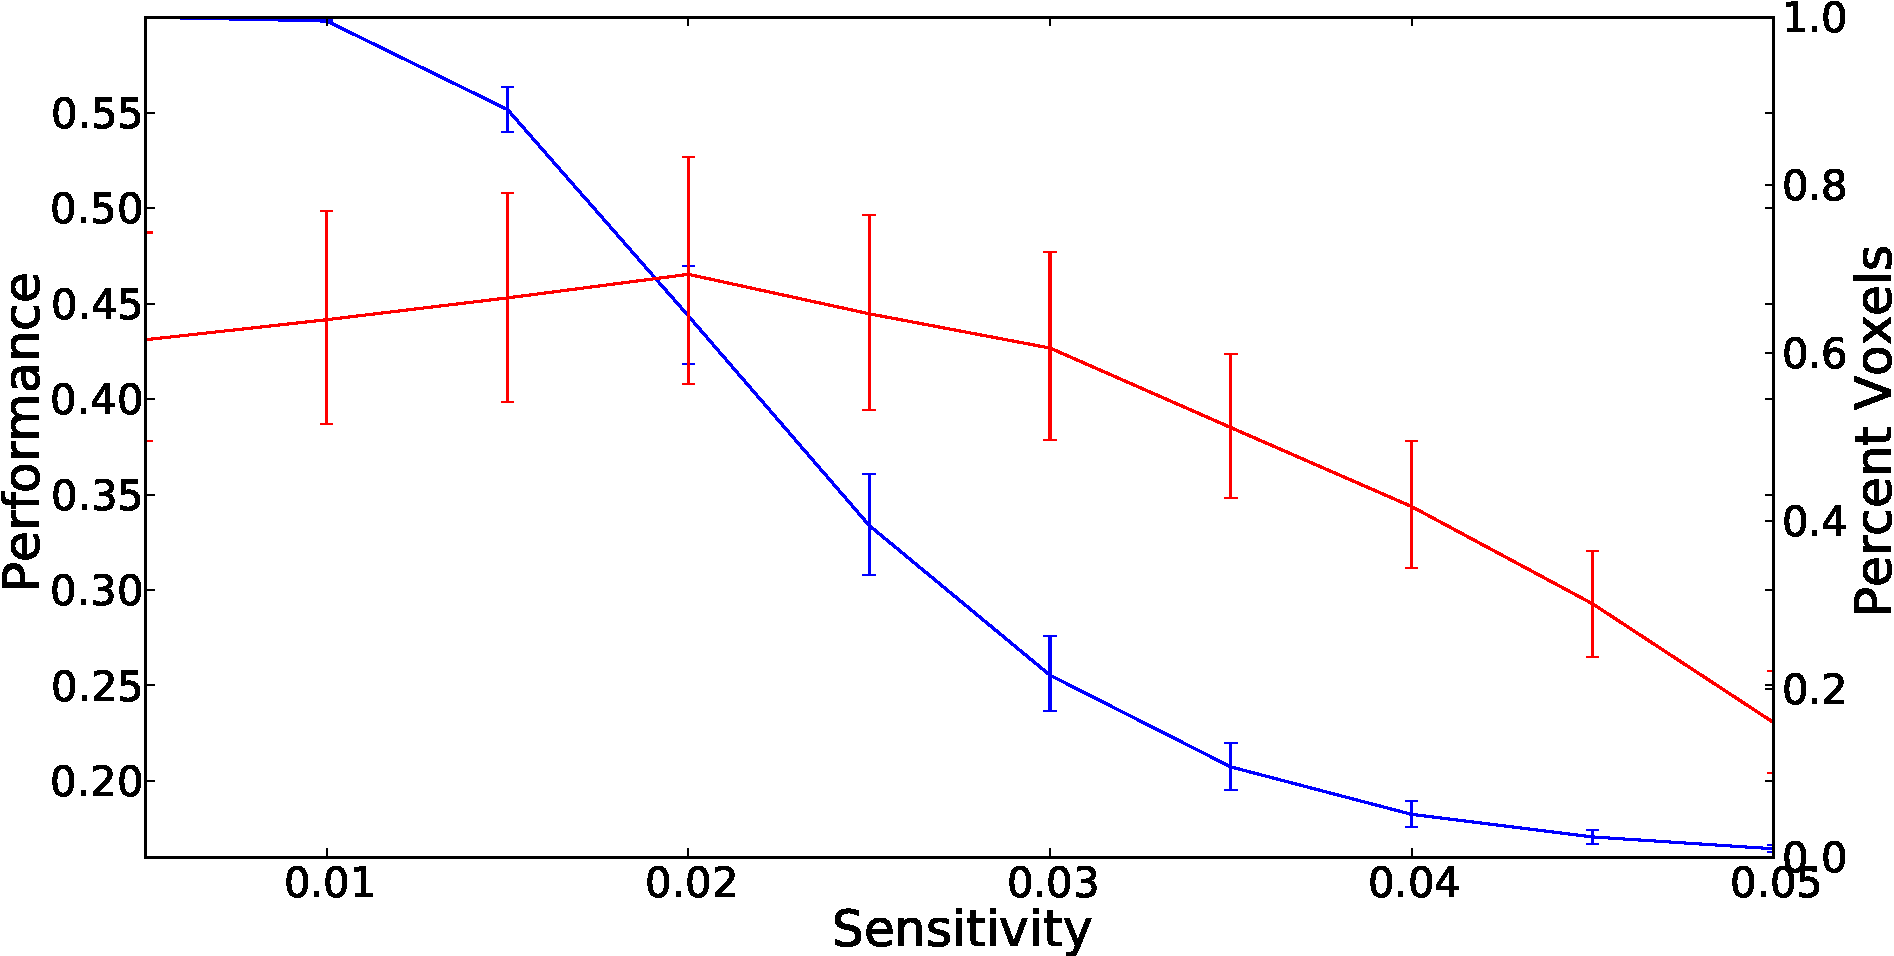
\includegraphics[width=0.4\textwidth]{figures/performance-verse-sensitivity-cutoff}
\caption{A plot of the feedforward neural network estimated performance and the percent of voxels used for training when the inputs are pruned at a particular sensitivity value.
The fraction of voxels is calculated with respect to the 2000 voxels selected by harmonic analysis.
The performance estimates and voxel counts were bootstrapped across sessions in order to obtain 68\% confidence intervals.
The estimated performance is not significantly reduced until over 90\% of the voxels have been pruned.
Interestingly, low levels of pruning may actually improve performance (presumably by reducing noise), although this effect was not statistically significant in the current experiment.} 
\label{fig:sensitivity-cutoff}
\end{figure}

Sensitivity maps for individual subjects show a preponderance of classification sensitivity in lateral occipital areas, ventral retinotopic early visual areas, and dorsal parietal lobe (Figure \ref{fig:individual-sensitivity}). 
The Z-statistic maps produced by GLM also indicate significant correlation between the magnitude of activation and character count in ventral retinotopic early visual areas and lateral occipital regions.
Individual subjects also displayed small regions of high sensitivity in idiosyncratic portions of temporal and frontal cortex. 
Averaged across subjects, classifier sensitivity was most affected (in order of importance) by lateral occipital regions, lingual areas, and dorsal parietal lobe (Table \ref{tab:full-sensitivity}). 

\begin{figure*}
\centering
\small{\input{surface-maps.pdf_tex}}
\caption{Sensitivity and GLM linear-response Z-statistic maps projected onto semi-inflated cortical surfaces for three different subjects.
The sensitivity and Z-score maps are roughly similar across subjects and hemispheres, but substantial individual variations are evident.}
\label{fig:individual-sensitivity}
\end{figure*}

\section{Discussion}

\begin{table*}
\centering

\begin{tabular}{cccccccc}
\toprule
Region & A & B & C & D & E  & Mean & Confidence Interval\\
\midrule
right lateral occipital & 26.54 & 13.41 & 16.26 & 24.17 & 26.49 & 21.37 & 18.76--23.98 \\
left lateral occipital & 13.37 & 25.65 & 15.37 & 24.02 & 25.75 & 20.83 & 18.37--23.28 \\
left superior parietal & 3.36 & 0.33 & 3.66 & 3.85 & 6.11 & 3.46 & 2.76--4.26 \\
left inferior parietal & 2.88 & 5.43 & 7.08 & 5.47 & 5.36 & 5.24 & 4.73--5.78 \\
right lingual & 6.64 & 5.96 & 10.30 & 5.88 & 5.25 & 6.81 & 5.93--7.69 \\
right superior parietal & 3.12 & 5.98 & 2.54 & 7.14 & 4.87 & 4.73 & 3.93--5.53 \\
right inferior parietal & 1.76 & 6.96 & 0.81 & 1.68 & 4.56 & 3.16 & 2.12--4.21 \\
left pericalcarine & 7.07 & 0.29 & 2.29 & 3.79 & 3.87 & 3.46 & 2.45--4.49 \\
left lingual & 8.63 & 8.38 & 10.09 & 4.92 & 3.50 & 7.10 & 6.07--8.37 \\
right superior temporal & 0.91 & 0.83 & 0.98 & 2.18 & 2.62 & 1.50 & 1.16--1.85 \\
right middle temporal & 0.23 & 0.84 & 6.08 & 1.69 & 2.54 & 2.28 & 1.28--3.27 \\
right pericalcarine & 4.64 & 5.99 & 6.02 & 0.40 & 2.20 & 3.85 & 2.82--4.91 \\
left superior temporal & 3.15 & 0.00 & 1.72 & 2.17 & 1.82 & 1.77 & 1.34--2.23 \\
right fusiform & 2.43 & 3.42 & 3.19 & 3.51 & 1.42 & 2.79 & 2.43--3.17 \\
right cuneus & 0.77 & 4.89 & 1.36 & 0.12 & 1.24 & 1.68 & 0.86--2.51 \\
left cuneus & 2.60 & 4.15 & 2.11 & 0.13 & 0.85 & 1.97 & 1.31--2.63 \\
left inferior temporal & 0.04 & 0.00 & 0.46 & 0.66 & 0.83 & 0.40 & 0.24--0.55 \\
right inferior temporal & 3.65 & 1.44 & 0.96 & 3.43 & 0.64 & 2.02 & 1.43--2.58 \\
left fusiform & 2.67 & 1.12 & 6.24 & 4.48 & 0.08 & 2.92 & 1.89--3.94 \\
left middle temporal & 5.53 & 4.93 & 2.51 & 0.33 & 0.00 & 2.66 & 1.62--3.70 \\
\bottomrule
\end{tabular}

\caption{Sensitivity map values integrated across the cortical surface labels. Sensitivities are shown for each subject (\emph{A}--\emph{E}), and their mean values, as shown ordered from greatest to least sensitive brain region.}
\label{tab:full-sensitivity}
\end{table*}

Although all classifiers performed at well above chance levels for all subjects, the average performance of individual subjects and the performance between sessions varied significantly (Figure \ref{fig:performance}).
These variations could be the result of differences in age, general cognitive state, or simply how much attention the subject was paying to the stimulus during a session.
The lack of a task during the stimulus presentation makes these variations difficult to interpret since attention and cognitive state were not well controlled.
In future experiments, the subjects will be asked to perform a challenging task, and the average performance is expected to increase and the variation between subjects to decrease.

In general, the classification accuracy of a particular number of presented human characters decreased as the number of characters increased (Figure \ref{fig:average-confusion}).
This observation is in agreement with the logarithmic nature of perception; i.e., it is easier to tell the difference between one and two characters than it is to tell the difference between five and six characters \citep{Shepard1975,Dehaene2003}.
This phenomenon could also be related purely to retinotopic information, as suggested by the GLM Z-score maps, rather than the perception of numbers.
Without a fixation point and with varying character group configurations, the retinotopic pattern of activation will vary from presentation to presentation even for the same character count.
However, the average activation in a retinotopically organized and object-selective region will increase for larger group sizes regardless of the group's configuration and the subject's fixation point.
The relative difference in average activity is smaller between larger presentation sizes and thus more difficult to differentiate.
However, there is a significant increase in confusion between two and six characters which is difficult to account for with a retinotopic explanation.
This could be a result of six characters being too much for the subject to consider individually, and the subject may sometimes encode two groups of characters rather than six individual characters.

The classifier performances validate the popularity of the SVM for MVPA.
In general, better classifier performance leads to higher confidence in the results of MVPA.
Therefore, it is important to identify new classification algorithms that could offer superior performance.
Deep learning \citep{Hinton2006} is a recent neural network formulation that has shown potential for solving a variety of complex tasks \citep{Ciresan2012}.
Discounting the two sessions with chance performance on the feedforward neural network, the performance of the NN was nearly identical to the SVM which suggests that deep learning could outperform even the SVM.
The poor performance of the NN on these two sessions may be due to the stochastic nature of NN training: The network possibly was not given enough time to converge to a good solution.

The classifiers' performance indicates that there is sufficient information in the pattern of BOLD signals to decode character count in a freely viewed stimulus. 
The results of the sensitivity analysis suggest that the neural substrates that encode such information are distributed across a number of visual areas.
However, a lack of sensitivity in an area does not imply that no information is encoded there.
Voxels with redundant or noisy information will exhibit low sensitivity.
Neural responses themselves can show strong spatial correlations on the centimeter scale, particularly in the higher order visual areas that dominate the sensitivity results \citep{Engel1997}. 
Voxels sampling these regions will contain useful but highly redundant information and will have a commensurately lower sensitivity.
As the pruning process proceeds, noisy and redundant voxels will be removed, thus reducing the redundancy of the remaining voxels and therefore boosting their sensitivity.
The resulting set of voxels will be highly reliable with very little redundant information.

Sensitivity analysis was only performed on the feedforward neural network classifier because of the existing literature on the topic \citep{Zurada1994}.
Applying a similar technique to the SVM is an avenue for future research.
When examined in conjunction with existing vision and cognitive neuroscience experiments, the sensitivity maps suggest how this information may be processed in the brain (Table \ref{tab:full-sensitivity}).
By far, the most sensitivity (42\%), and therefore the most relevant mutual information, is contained in the lateral occipital region (LO).
This region is most commonly associated with high-level object recognition \citep{Grill-Spector2001}, but also contains the extrastriate body area which has been implicated in the perception of body parts \citep{Astafiev2004}.
This observation is in contrast to the comparatively weak sensitivity (5.7\%) observed in the fusiform gyrus, which is also associated with object classification tasks and in particular the perception of human faces \citep{Kanwisher1997,Sayres2010}.
The superior temporal sulcus (STS), which has also been implicated in object selectivity \citep{Hasselmo1989,Beauchamp2004}, also contained some sensitivity. 

Additionally, there is substantial sensitivity contained in low-level retinotopic visual areas. 
The pericalcarine, lingual, and cuneus areas altogether account for 25\% of the observed sensitivity; the more ventral lingual areas contribute more strongly (13.9\%) then cuneus (3.7\%).
This result is somewhat surprising given that the relevant information in the scene is not obviously retinotopically organized due to the randomized arrangement of buildings and characters as well as the free-viewing paradigm.
However, the classification sensitivity and significant correlation between magnitude of activation and character count in early retinotopic visual areas and the sensitivity in lateral-occipital areas suggests that retinotopic organization is important in decoding group size. 
Because LO combines object-selectivity with retinotopic specificity \citep{Sayres2008}, different group sizes could evoke complex but stereotypical patterns of responses in LO (and other retinotopically organized areas) as subjects visually interrogate the stimuli with a sequence of eye movements. 

Despite the preponderance of retinotopic visual-area sensitivity, the dorsal parietal cortex also shows substantial sensitivity (16.6\%).
Regions in the parietal cortex have been shown to be involved in mental arithmetic and magnitude judgement \citep{Rickard2000} which may also play some role in decoding group size.
More recent research suggests this region may even contain a topographic representation of numerosity \citep{Harvey2013}.
There is some debate as to whether this topographic map represents numerosity or sensory processing \citep{Gebuis2013}, but it would be useful for decoding group size regardless. 
The relatively small sensitivity that we observe from this region could be the consequence of its small size and our limited spatial resolution; higher sensitivity in this region may be available at higher spatial resolutions.

The maps of significant correlation between magnitude of activation and character count produced by a GLM are predominately observed in early retinotopic visual areas as well as lateral occipital and fusiform regions.
In general, these maps covered only a small subset of those regions found to be sensitive by MVPA.
Thus MVPA delineates a more distributed neural substrate for the encoding of character count, and also performs significantly better than a simple linear estimator.
These differences suggest that the performance of the MVPA can only be partially explained by simple linear and retinotopically organized activation.
By modeling the higher level visual areas indicated by the sensitivity analysis, it should be possible to improve the performance of the model-based estimator.
This process illuminates a strategy for moving from flexible yet difficult to interpret machine-learning results to well-understood models that are amenable to testing with a GLM.

While virtual environments offer a more realistic stimulus than traditional stimuli such as sweeping bars or contrast gratings, they are more complex to design and more difficult to interpret.
This paper offers some initial tools and analyses to deal with these challenges, but further work is needed to explore the application of these techniques in richer virtual environments.
It should also be noted that virtual environments do carry some disadvantages over simpler dynamic stimuli such as prerecorded movies. 
It is typically easier to record a movie than to program a virtual environment; movies can also have a more realistic appearance than virtual environments.
Additionally, the results of \cite{Han2005} indicate that there is some divergence in the way the brain processes real (i.e., recorded) and virtual visual worlds. 
However, it is likely that this divergence in processing will decrease as the realism of virtual environments increases.

Complex and dynamic stimuli allow researchers to examine neural processing in a more natural state, and virtual environments make it easier to design and control such stimuli.
MVPA allows researchers to explore the coding of information in the brain when an underlying neural processing model is not already known and to discover new and interesting interactions.
Used together, virtual environments and MVPA allow for novel and valuable experimental designs.
Altogether, the results in this paper suggest that the combination of virtual environments with machine-learning analysis schemes will offer a fruitful new tool for the analysis of brain responses in stimulus scenarios that more closely resemble natural human experience.

\section{References}
\bibliography{bib}

\end{document}
